%The workload of a typical MCU might consist of hundreds of tasks with variable lengths, which are queued to the two cores, creating two large task bins in each one of them. In order to attenuate the complexity that such an approach would introduce, we decided to use a task abstraction. Instead of having multiple tasks, which are merged to create a large task bin in each core, we assumed that we have only two tasks from the beginning, that need to be allocated to two cores. This abstraction simplified the derivation of the allocation policies and the conduction of the experiments, without altering the final conclusions.\par
The application consists of a set of \textit{n} periodic tasks. It is assumed that all tasks have the same period $D$. Furthermore, it is assumed that all tasks are atomic units of execution; therefore, preemptions and migrations are not allowed. This is a fairly restrictive assumption; however, it is realistic for deeply low power MCU platforms. $C_i$ is used to denote the computation cycles of task $i$.


%During our experiments, we used tasks with a constant period, defined in terms of clock cycles. Furthermore, due to the lack of high-level techniques such as preemption and migration in MCUs, our tasks are atomic units of execution. This is actually very restrictive, because as you can see in Figure~\ref{fig:task_model}, when we have two tasks with very different sizes, then the makespan does not improve significantly.\par

%\begin{figure}[!htbp]
%  \centering
%  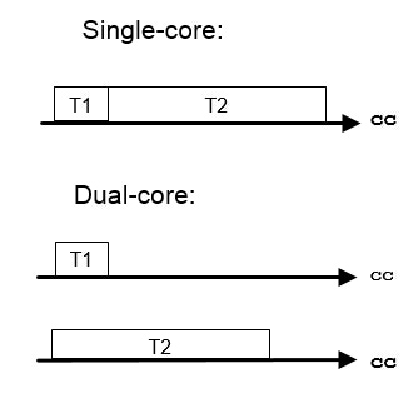
\includegraphics[scale=0.6]{./figures/task_model}
%  \caption{Tasks with high variability}
%  \label{fig:task_model}
%\end{figure}

%In order to test different levels of parallelism, we introduced the \emph{computation cycle variation ($\Delta)$}, which shows the fractional difference from the mean computation cycles ($C_{mean}$). For example, when $\Delta = 0$, it means both tasks need the same number of computation cycles. When $\Delta = 0.5$, it means tasks are $\pm50\%$ from the mean. So, we can calculate the time that each core needs in order to execute a task as following:

%\begin{align} 
%A_{HC} = \frac{C_{mean}\times\left(1\pm\Delta\right)}{F_{HC}} \\ 
%A_{LC} = \frac{C_{mean}\times\left(1\pm\Delta\right)}{F_{LC}}
%\end{align}

%, where $C_{mean}\times\left(1+\Delta\right)$ are the computation cycles of the large task and $C_{mean}\times\left(1-\Delta\right)$ the computation cycles of the small task.
%%% Local Variables: 
%%% mode: latex
%%% TeX-master: "../report_template"
%%% End: 
